% Research proposal: extension of "Consolidate, then Gate" (continual learning of manipulation skills in a VLA).
% Structure: NSF Project Summary (Overview, Intellectual Merit, Broader Impacts) and Project Description (PAPPG 24-1,
% Chapter II.D.2), condensed.
% Build: tectonic -X compile proposal.tex   (figure: python docs/proposal/make_figures.py, see its docstring)
\documentclass[11pt]{article}
\usepackage[letterpaper,margin=0.6in]{geometry}
\usepackage[T1]{fontenc}
\usepackage{tgheros}
\renewcommand{\familydefault}{\sfdefault}
\usepackage{amsmath}
\usepackage{microtype}
\usepackage{graphicx}
\usepackage{booktabs}
\usepackage[table]{xcolor}
\usepackage{tikz}
\usetikzlibrary{arrows.meta,fit,calc}
\usepackage{enumitem}
\usepackage{multicol}
\usepackage[font=small,labelfont=bf,skip=3pt]{caption}
\usepackage{titlesec}
\usepackage[numbers,sort&compress]{natbib}
\usepackage[colorlinks=true,linkcolor=linkblue,citecolor=linkblue,urlcolor=linkblue]{hyperref}

\definecolor{linkblue}{HTML}{1F5FAD}
\definecolor{ink}{HTML}{121211}
\definecolor{ink2}{HTML}{52514E}
\definecolor{coreA}{HTML}{2A78D6}
\definecolor{coreB}{HTML}{6250D6}
\definecolor{free}{HTML}{D6E8C4}
\definecolor{inp}{HTML}{F1F0EC}
\definecolor{goal}{HTML}{E3ECFA}
\definecolor{sens}{HTML}{FDEDE1}
\definecolor{fail}{HTML}{B4246A}
\definecolor{oursrow}{HTML}{EAF2FC}
\definecolor{summary}{HTML}{F5F4F0}

\setlength{\parindent}{0pt}
\setlength{\parskip}{3.5pt}
\titleformat{\section}{\large\bfseries}{}{0pt}{}
\titlespacing*{\section}{0pt}{4pt}{1pt}
\titleformat{\subsection}{\normalsize\bfseries}{}{0pt}{}
\titlespacing*{\subsection}{0pt}{4pt}{0pt}
\titlespacing*{\paragraph}{0pt}{3pt}{0.6em}
\setlist{nosep,leftmargin=1.1em}
\setlength{\bibsep}{0.5pt}
\renewcommand{\bibfont}{\scriptsize}
\setlength{\textfloatsep}{8pt}
\setlength{\floatsep}{6pt}
\setlength{\emergencystretch}{1.5em}
\renewcommand{\bibsection}{\section*{References cited}}

\begin{document}

\begin{center}
{\Large\bfseries Contextual Motor Memory for Continual Robot Learning:\\[1pt]
Selective Consolidation, Skill Retrieval and Physical Adaptation}\\[3pt]
{\small Research proposal extending \emph{Consolidate, then Gate}
(\href{https://github.com/DishengTang/continual_vla}{github.com/DishengTang/continual\_vla})}
\end{center}
\vspace{-8pt}
\suppressfloats[t]

\section*{Project Summary}
\noindent\colorbox{summary}{\parbox{\dimexpr\linewidth-2\fboxsep\relax}{\small
\textbf{Overview.} Robots that work alongside people must keep adding skills without losing earlier ones. Pretrained
vision-language-action (VLA) policies forget earlier skills when fine-tuned in sequence unless a share of every task's
data is kept for replay or training is restricted. This project develops a \emph{contextual motor memory} for VLA policies, modelled on how brains store and
select motor skills: each skill is consolidated into a compact set of protected units of the policy's action network,
retrieved by inferring the requested goal and the physical context, and capacity is reallocated as skills accumulate.
Aim~1 determines when and why pretrained robot policies forget; Aim~2 develops the memory from a prototype that,
without stored data, matches or exceeds replay and PackNet at small allocations; Aim~3 tests it on a real arm.\\[2pt]
\textbf{Intellectual Merit.} The project separates three causes of apparent forgetting, lost storage, failed retrieval
and changed physical conditions, which need different remedies; locates the computations each skill relies on by causal
intervention; and turns principles of engram allocation, graded synaptic consolidation, systems consolidation and
contextual inference into a continual learner whose memory does not grow with stored data and whose capacity is
recycled rather than exhausted.\\[2pt]
\textbf{Broader Impacts.} Robots could learn new tasks on site without keeping their users' demonstrations, lowering
storage cost and privacy risk; code, benchmarks and protocols for a low-cost open-source arm will be released, and the
project trains students across robot learning and neuroscience.}}

\section*{Project Description}

\subsection*{1. Introduction and objectives}
Brains keep motor skills with bounded resources: skills are stored in skill-specific sets of synapses whose erasure
removes one skill and spares another \citep{hayashitakagi2015}, and the current context is inferred to decide whether a
motor memory is expressed, updated or newly created \citep{heald2021}. A prototype built on these principles,
consolidate-and-gate, kept three manipulation skills in a pretrained VLA without storing earlier data (\S3), but it
reserves a fixed, frozen share of the network for each skill and stops learning once the network is full.

\textbf{Central hypothesis:} \emph{forgetting in pretrained robot policies decomposes into failures of storage,
retrieval and physical adaptation, and a contextual motor memory, whose skill cores are allocated by need, protected in
proportion to their use and retrieved by the inferred goal and physical context, preserves reliable execution as skills
accumulate under bounded memory and capacity} (Fig.~\ref{fig:framework}). Three aims test it:

\textbf{Aim 1. Determine when and why pretrained robot policies forget.} \emph{Outcome:} a map of the regimes that need
structural protection, separating lost skills from unretrieved ones.\\
\textbf{Aim 2. Develop a contextual motor memory that keeps learning after the network is full.} \emph{Outcome:} the
prototype's retention for many more skills at a fixed capacity, without stored demonstrations.\\
\textbf{Aim 3. Demonstrate sequential learning, retrieval and physical adaptation on a real arm.} \emph{Outcome:} a
physical test of retention and context inference, measured by reliability, wrong-goal actions and human interventions.

\begin{figure}[b]
\centering
\begin{tikzpicture}[font=\sffamily\scriptsize, >={Stealth[length=4pt]},
  box/.style={draw=ink, line width=0.6pt, rounded corners=3pt, align=center, inner sep=2.5pt},
  arr/.style={->, line width=0.6pt, draw=ink2},
  failmark/.style={circle, fill=fail, text=white, font=\sffamily\scriptsize\bfseries, inner sep=0.8pt, minimum size=10pt}]
  % inputs
  \node[box, fill=inp, minimum width=2.75cm] (img) at (0,1.45) {Camera image};
  \node[box, fill=inp, minimum width=2.75cm] (jnt) at (0,0.85) {Joint angles};
  \node[box, fill=inp, minimum width=2.75cm] (ins) at (0,0.05) {Instruction\\\textit{``stack the green cube on red''}};
  \node[box, fill=inp, minimum width=2.75cm] (his) at (0,-0.95) {Interaction history\\(recent observations, actions)};
  % context inference
  \node[box, fill=goal, minimum width=3.0cm] (goalc) at (4.05,0.55) {\textbf{Goal context}\\read from the instruction};
  \node[box, fill=sens, minimum width=3.0cm] (sensc) at (4.05,-0.6) {\textbf{Sensorimotor context}\\inferred by an action-\\conditioned predictor};
  \node[draw=ink2, dashed, rounded corners=4pt, fit=(goalc)(sensc), inner sep=4pt] (ctx) {};
  \node[font=\sffamily\scriptsize\bfseries, anchor=north] at (ctx.south) {Context inference};
  \draw[arr] (ins.east) -- (goalc.west);
  \draw[arr] (his.east) -- (sensc.west);
  % gate
  \node[box, fill=white, minimum width=1.0cm] (gate) at (6.75,0) {Gate:\\select\\cores};
  \draw[arr] (goalc.east) -- (gate.north west);
  \draw[arr] (sensc.east) -- (gate.south west);
  % action expert: skill cores (some units shared by compatible skills) and plastic units
  \def\gx{7.75} \def\gy{-0.75} \def\cs{0.3}
  \foreach \i in {0,...,9} { \foreach \j in {0,...,4} {
      \pgfmathtruncatemacro{\k}{mod(\i*7+\j*3,10)}
      \ifnum\k<2 \def\col{coreA}\else\ifnum\k<3 \def\col{coreA!50!coreB}\else\ifnum\k<4 \def\col{coreB}\else\def\col{free}\fi\fi\fi
      \fill[\col] (\gx+\i*\cs, \gy+\j*\cs) rectangle ++(0.25,0.25);
  } }
  \node[draw=ink, line width=0.6pt, rounded corners=3pt, fit={(\gx-0.08,\gy-0.08) (\gx+10*\cs,\gy+5*\cs)}, inner sep=1pt] (expert) {};
  \node[font=\sffamily\scriptsize\bfseries, anchor=south] at (expert.north) {Action expert};
  \node[font=\sffamily\tiny, anchor=north, align=center, text=ink2] at (expert.south) {\textcolor{coreA}{\rule{4pt}{4pt}}\,\textcolor{coreB}{\rule{4pt}{4pt}} skill cores\quad \textcolor{coreA!50!coreB}{\rule{4pt}{4pt}} shared\quad \textcolor{free!70!black}{\rule{4pt}{4pt}} plastic};
  \draw[arr] (gate.east) -- (expert.west |- gate.east);
  \draw[arr] (img.east) -- ++(0.35,0) |- ($(expert.north west)+(0.6,0.42)$) -- ($(expert.north west)+(0.6,0.02)$);
  \draw[line width=0.6pt, draw=ink2] (jnt.east) -- ++(0.35,0) -- ($(img.east)+(0.35,0)$);
  % outputs and world
  \node[box, fill=inp, minimum width=1.55cm] (act) at (12.35,0) {Action chunk};
  \node[box, fill=inp, minimum width=2.3cm] (world) at (14.85,0) {Arm and objects\\(surface, payload)};
  \draw[arr] (expert.east |- act.west) -- (act.west);
  \draw[arr] (act.east) -- (world.west);
  \draw[arr] (world.south) -- ++(0,-1.5) -| (his.south);
  % failure points
  \node[failmark] at (expert.north east) {S};
  \node[failmark] at ($(gate.east)!0.5!(expert.west |- gate.east)+(0,0.22)$) {R};
  \node[failmark] at (world.north east) {P};
\end{tikzpicture}
\caption{\textbf{Contextual motor memory.} The policy reads the goal from the instruction and infers the physical
context from its interaction history; a gate runs the cores of the inferred skill, shared by compatible skills and
protected in proportion to their use, while other units stay plastic. A skill that seems forgotten can fail at storage
(S: its computation is overwritten), retrieval (R: the wrong core is selected) or physical adaptation (P: the dynamics
change under the same goal).}
\label{fig:framework}
\end{figure}

\subsection*{2. Background and relation to current knowledge}
\paragraph{When pretrained VLA policies forget.} Sequential supervised fine-tuning erases earlier skills in $\pi_0$ and
GR00T N1.5 (negative backward transfer, NBT, 0.56--0.76 on LIBERO) \citep{liu2026pretrained}, $\pi_{0.5}$ (86.9\% to
31.4\% average success on a real task stream) \citep{zhu2026realworld}, OpenVLA-OFT (NBT 78.7\%) \citep{hu2026simple} and
compact pretrained policies \citep{romer2026clare,gu2026limode}, and erodes a generalist's broader skills
\citep{yadav2026retain}. The finding that pretrained VLAs resist forgetting \citep{liu2026pretrained} rests on replaying
15--20\% of each task's data; with 2\% the NBT is 0.12--0.18, and with 0.2\% 0.58--0.75. On real data 2\% suffices once
the replay ratio and action normalization are tuned \citep{zhu2026realworld}, and on-policy reinforcement learning with
LoRA forgets little, but 40.9\% without LoRA \citep{hu2026simple}. Retention thus depends on replay, objective and update
scope, and has been shown for tasks that differ mostly in scene or objects, not without a growing store of
demonstrations, for goals that demand opposite actions in one scene, or under changed physical conditions. Forgotten skills recover within 6--11\% of their original training \citep{liu2026pretrained}, suggesting
that a skill can remain stored but unexpressed; without a control that never learned the skill, however, recovery
cannot be told apart from fast learning.

\paragraph{Isolation and routing.} Structural methods reserve parameters per task by weight magnitude
\citep{mallya2018packnet} or learned masks \citep{serra2018hat}, or add adapters and experts with routers
\citep{liu2024tail,lei2025dmpel,romer2026clare,gu2026limode}. Fixed reservations
exhaust the network, added modules grow with every task, and none measures which computations a skill relies on, lets
compatible skills share protected units, or tells a lost skill from an unretrieved one. Generated replay with
world-action models avoids stored data \citep{govind2026regen,fang2026r2wam,lin2026rifar} but adds generation cost, and video
can stay plausible while actions fail \citep{fang2026r2wam}.

\paragraph{Principles from neuroscience.} Memories are allocated to the neurons most excitable at learning, and
memories formed close in time share neurons \citep{josselyn2020,cai2016}; graded, multi-timescale synaptic consolidation
stores far more memories than binary synapses \citep{benna2016}; memories move from fast hippocampal to slow cortical
storage \citep{mcclelland1995}; and contextual inference decides which motor memory is expressed or updated
\citep{heald2021}. Context-dependent gating brought skill-specific units into
networks given a task signal \citep{masse2018}; together, these principles are untested in robots.

\subsection*{3. Preliminary results}

\begin{figure}[t]
\centering
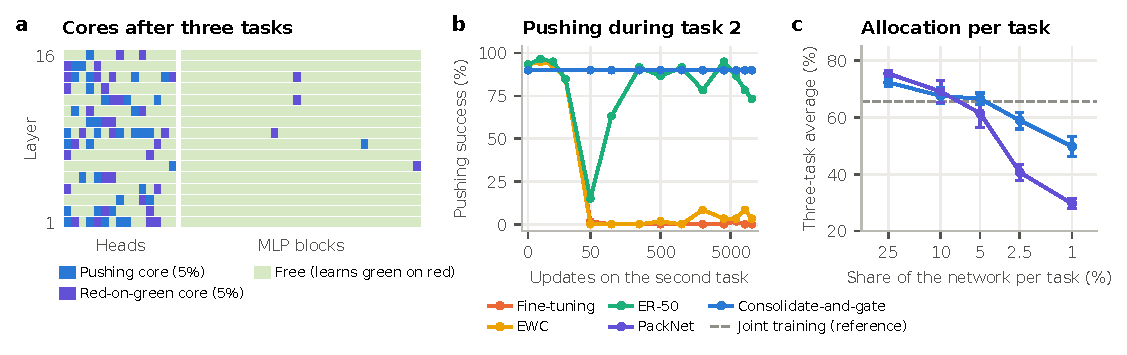
\includegraphics[width=\linewidth]{fig_results.pdf}
\caption{\textbf{Preliminary results} (SmolVLA, ManiSkill~3; 3 training seeds). \textbf{a,} Seed-0 cores among the 752
unit groups of the action expert after three tasks: pushing runs only its core, red on green both cores, and green on
red, the newest task, every group. \textbf{b,} Pushing success while stacking red on green is learned; validation
scenes, mean of seeds. \textbf{c,} Three-task average against the share of the network reserved per task; 100 test
scenes per task, mean $\pm$ SD.}
\label{fig:results}
\end{figure}

SmolVLA (0.45B parameters; frozen vision-language backbone, 100M-parameter action expert) \citep{shukor2025smolvla}
learned pushing, stacking red on green, and the opposite stack in the same ManiSkill~3 scenes \citep{tao2025maniskill3}
from demonstrations, seeing only a camera image, its joint angles and the instruction. Fine-tuning lost pushing within
50 updates of the second task (Fig.~\ref{fig:results}b) and later built the newest stack for 63.0\% of red-on-green
requests; replaying 500 examples of each earlier task, 0.5\% of the stacking data, kept pushing but only 28.3\% of
red-on-green stacks, as in the small-buffer regime above (Table~\ref{tab:three}). The prototype retrains each learned
skill in a random 5\% of the action expert's 752 unit groups (heads and 64-neuron MLP blocks), silences the others for
that skill's instruction and freezes the core (Fig.~\ref{fig:results}a). Without the gate, pushing fell
from 93.3\% to 0.3\%; without freezing, to 0.0\%. After three tasks it averaged 66.6\% with 188 bytes of masks and no
earlier data, ahead of PackNet \citep{mallya2018packnet} at 5\%, 2.5\% and 1\% per task (Fig.~\ref{fig:results}c).

\begin{table}[h]
\centering
\caption{\textbf{Three-task results.} Success (\%) after all three tasks; 100 test scenes per task, mean $\pm$ SD over 3
seeds; each method at its best three-task configuration. ER-50/500: 50 or 500 stored examples per earlier task. Wrong
stack: green on red built when red on green was requested. Average: mean of the three tasks. Memory kept: replay
buffers, Fisher information and earlier weights (EWC), or one bit per weight (PackNet) or unit group (prototype) and
task.}
\label{tab:three}
\footnotesize
\setlength{\tabcolsep}{5pt}
\begin{tabular}{@{}lrcccccc@{}}
\toprule
Method & Memory kept & Pushing & Red on green & Wrong stack & Green on red (new) & Average \\
\midrule
Fine-tuning & none & 1.7 $\pm$ 1.2 & 0.0 $\pm$ 0.0 & 63.0 $\pm$ 1.7 & 64.7 $\pm$ 1.2 & 22.1 $\pm$ 0.4 \\
EWC \citep{kirkpatrick2017ewc} & 0.80 GB & 6.7 $\pm$ 4.7 & 1.3 $\pm$ 1.2 & 14.0 $\pm$ 2.6 & 13.3 $\pm$ 4.6 & 7.1 $\pm$ 2.6 \\
ER-50 & 19.7 MB & 80.3 $\pm$ 5.0 & 3.0 $\pm$ 2.0 & 14.0 $\pm$ 14.8 & 60.0 $\pm$ 2.0 & 47.8 $\pm$ 1.5 \\
ER-500 & 197 MB & 92.3 $\pm$ 3.1 & 28.3 $\pm$ 3.1 & 3.7 $\pm$ 1.5 & 58.7 $\pm$ 3.1 & 59.8 $\pm$ 1.7 \\
PackNet, 5\% per task & 25.0 MB & 85.3 $\pm$ 2.3 & 45.3 $\pm$ 3.2 & 0.0 $\pm$ 0.0 & 53.7 $\pm$ 9.1 & 61.4 $\pm$ 4.9 \\
\rowcolor{oursrow}\textbf{Consolidate-and-gate, 5\% cores} & 188 B & 93.3 $\pm$ 3.8 & 43.3 $\pm$ 4.2 & 0.0 $\pm$ 0.0 & 63.0 $\pm$ 7.0 & \textbf{66.6 $\pm$ 2.0} \\
\midrule
\textit{Joint training (reference)} & all data & 99.0 $\pm$ 0.0 & 48.3 $\pm$ 4.0 & 1.7 $\pm$ 0.6 & 49.0 $\pm$ 6.1 & 65.4 $\pm$ 0.7 \\
\bottomrule
\end{tabular}
\end{table}

\paragraph{Limitations that define Aim 2.} The prototype is deliberately simple and shares the rigidity of PackNet.
(i) Each skill takes a fixed, exclusive, frozen share, so the network is exhausted after a fixed number of skills;
PackNet overtakes it at 10\% and 25\% per task (Fig.~\ref{fig:results}c), and releasing half of each earlier core to
admit a third task lost red on green. (ii) Frozen cores can neither improve with new data nor adapt to new physical
conditions. (iii) Every skill gets the same random share, whatever its difficulty; a core chosen by intervention raised
the two-task average from 72.2\% to 75.0\%. (iv) The gate maps each instruction to a stored task label, so paraphrases,
new combinations of skills and changed physical conditions are not inferred.

\subsection*{4. Research plan}
\paragraph{Shared design.} \emph{Models:} SmolVLA; $\pi_0$ \citep{black2024pi0} to confirm the main findings.
\emph{Benchmarks:} LIBERO-Goal (ten goals, one scene) \citep{liu2023libero}, LIBERO sequences of 30--40 tasks
\citep{hu2026simple,romer2026clare}, and ManiSkill families of same-scene tasks with conflicting goals, scaled to tens
of tasks. \emph{Baselines:} fine-tuning, sequential and per-task LoRA \citep{liu2024tail}, tuned ER, EWC,
PackNet, CLARE, joint training and the prototype. \emph{Rigor:} selection on validation scenes, one evaluation on
untouched scenes, several task orders and seeds, full accounting of compute and storage. \emph{Metrics:} success, NBT, forward transfer, wrong-goal actions, memory per skill and skills admitted per capacity.

\paragraph{Aim 1: Determine when and why pretrained robot policies forget.} Around two anchors, our setting and that of
\citet{liu2026pretrained}, we will vary pretraining (SmolVLA versus $\pi_0$, each also initialized from its
vision-language model only), update scope (full action-expert fine-tuning versus sequential LoRA), objective (supervised
versus on-policy reinforcement learning \citep{hu2026simple}), replay (0--20\% of each earlier task) and goal conflict
(different scenes; one scene with different objects; the same objects in swapped roles), crossing the factors that
interact. Conflict is measured before training, from the overlap of two skills' gradients and unit activations, to test
whether it predicts forgetting. Oracle versus learned routing separates failed retrieval from lost storage; recovery is
tested by learning A, then B, then re-exposing A, against an A-naive policy given the same training. \emph{Decision point:} regimes where a small buffer or sequential LoRA suffices are reported and left aside; measured
conflict guides sharing in Aim 2.

\paragraph{Aim 2: Develop a contextual motor memory that keeps learning after the network is full.} Starting from the
prototype, four changes address its limitations. \emph{Allocation by need (iii):} a new skill's core
grows from a small seed of unit groups ranked by causal importance (silencing and activation patching), as
engrams go to the most excitable neurons \citep{josselyn2020}, until the core alone matches the
full policy on validation scenes. \emph{Shared, graded protection (i, ii):} units may serve several skills; instead of
freezing, each unit learns more slowly as the importance of the skills relying on it grows, as in multi-timescale
synaptic consolidation \citep{benna2016}, and updates to shared units are projected away from the inputs of stored
skills \citep{saha2021gpm}. Low-conflict skills (Aim 1) share units, and conflicting ones are kept apart
\citep{cai2016}, so cores can be refined without being overwritten. \emph{Capacity recycling (i):} when free capacity
runs low, cores of related skills are distilled into fewer shared units on states from closed-loop rollouts, analogous to
systems consolidation \citep{mcclelland1995}; retention is verified before freed units are reinitialized to
stay plastic \citep{dohare2024}. \emph{Inferred retrieval (iv):} a light router maps the instruction, including
paraphrases and new combinations of known skills, to a weighting over cores, and flags unfamiliar contexts, for which a
new core is created rather than an old one overwritten \citep{heald2021}. \emph{Evaluation:} streams of 10--40 skills at
a fixed total capacity, against the prototype, PackNet, per-task LoRA, CLARE and ER at matched memory, with each change
ablated. \emph{Success:} more skills admitted than by the prototype and PackNet at the same retention, without stored
demonstrations. \emph{Alternatives:} replay sized by Aim 1 if distillation loses skills; freezing if cores drift.

\paragraph{Aim 3: Sequential learning, retrieval and physical adaptation on a real arm.} An open-source SO-101 arm, on
which SmolVLA was demonstrated \citep{shukor2025smolvla}, and a Franka Panda where available learn pick-and-place,
placement into different containers by instruction, a conflicting placement rule and stacking; a new surface or payload
is then introduced under the same instruction, and later removed. A small action-conditioned latent predictor over
visual features, proprioception and recent actions, in the spirit of V-JEPA~2 \citep{assran2025vjepa2}, detects changed
dynamics and gives the router its sensorimotor context. \emph{Hypothesis:} the adaptation is stored as a context-specific
variant of the skill's core rather than overwriting it, so the original behavior returns with the original conditions,
as contextual inference predicts for human motor learning \citep{heald2021}. \emph{Measures:} completion, wrong-goal
actions, interventions, recoveries, adaptation trials and latency. \emph{Extension:} for world-action models
\citep{ye2026dreamzero}, protecting the action computation, the predictive computation or both is compared with
generated replay \citep{govind2026regen,fang2026r2wam,lin2026rifar}.

\subsection*{5. Broader impacts}
Robots that learn on site without keeping their users' demonstrations lower storage cost and privacy risk and need less
retraining, which matters most for small laboratories and firms. Code, task families, trained cores and protocols will
be released for a low-cost open-source arm that classrooms can reproduce. Testing theories of motor memory in embodied
agents links robot learning with neuroscience and trains students in both fields.

\begin{multicols}{2}
\bibliographystyle{unsrtnat}
\bibliography{references}
\end{multicols}

\end{document}
